\documentclass[12pt]{article}

% import packages
\usepackage[utf8]{inputenc}
\usepackage{float}
\usepackage{subfloat}
\usepackage{subfig}
\usepackage{amsmath}
\usepackage[toc,page]{appendix}
\usepackage{caption}
\usepackage{graphicx}
\usepackage{hyperref}

\graphicspath{ {./images} }
% hyperref setup
\hypersetup{
	colorlinks=true,
	linkcolor=blue,
	filecolor=blue,      
	urlcolor=blue,
	citecolor=blue,
	pdftitle={Investigation into vehicle motion measurement techniques},
	pdfpagemode=FullScreen,
}
% titlepage	
\title{\textbf{Investigation into vehicle motion measurement techniques}}
\author{Callum Stephenson, css47, GRP173, Car4, Trinity}
\date{}

\begin{document}
    \begin{titlepage}
        \maketitle
        \thispagestyle{empty}
        \vspace{13cm}
        \textbf{Department of Engineering, University of Cambridge}
    \end{titlepage}
    \tableofcontents
    \newpage
    \section{Introduction}
    The aim of this report is to determine which techniques for analysing vehicle motion are most accurate, as well as 
    understanding how they are able to track a specific quantity about the vehicle. 
    
    Within this report, a model 1:18 488 GTB equipped with sensors will be used in order to investigate the performance of
    different sensors on the car. Being able to track the motion of a vehicle accurately is useful when trying to determine path,
    or to change certain values within the engine to increase effiency or maintain a set speed. One aspect to accuracy is the calibration of
    a measurement device between digital and real world steps. This is done on the model vehicle within this experiment similarly to
    how one might calibrate e-steps on a 3D printing machine by counting the movement in the axis comparative to rotation in the stepper motor.
    \newpage
    \section{Figures, answers to questions \& bullet points}
    \subsection{Figure 1}
    \begin{figure}[H]
    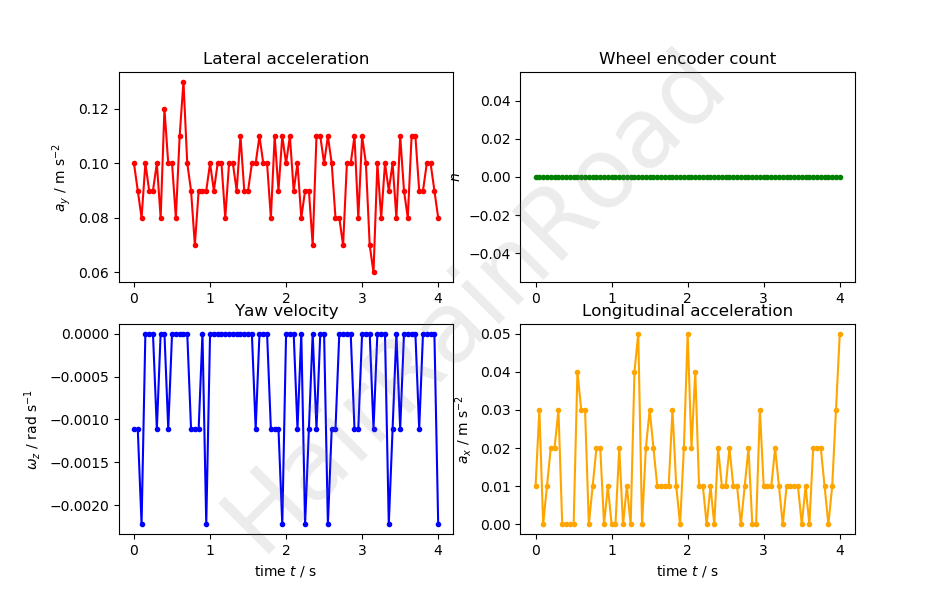
\includegraphics[width=35pc]{fig1png.png}\label{figure1}
    \caption{}
    \end{figure}
    \section{Conclusion}
    \begin{thebibliography}{99}
        
    \end{thebibliography}
\end{document}